% ********** Software platform **********

\chapter{Software platform}

The software that runs on the Sparrowv3 nodes and the SparrowDongle was
developed by As. Drd. Ing. Andrei Voinescu and is dubbed the SparrowLibrary.
In the process of implementing this protocol we have greatly improved not only
its functionality but its stability and user-friendliness.

The main focus of this library is to provide a C interface for working with the
Sparrow nodes and dongle. It must also be compatible with past and future
Sparrow devices, thus it must support multiple platforms and do this in a
scalable manner. To this end we divided the library into board and platform
sections.  Each device must declare exactly one board and one platform, with
the board defining the physical components that make up the device (sensors,
LEDs etc.) and the platform defining the microcontroller (ADC, timers etc.). 

In order to facilitate switching between different devices we used a
cross-platform build system (CMAKE) and divided the library into modules. The
build system allows the user to select the device that his/her code is to be
compiled for and Makefiles will be automatically generated to suit while
modularization of the library means that new code can be easily added to it, all
of this while keeping the compilation process fast and the resulting code
efficient.

Next we will present some of the most important modules and their
implementation.

\section{Radio}

This module allows the user to enable the ATmega128RFA1 radio transceiver and
use it in either a non-interactive or an interactive way. 

The interactive interface consists of a series of functions that can be called
to manipulate the device. They allow the user to put the transceiver into 
sleep state or into active mode, check its availability to accept new
commands, transmit and receive a frame (both blocking and non-blocking).

The programmer can also choose to work with the radio in a non-interactive
manner. This is achieved through four callbacks that can be passed to the
initialization function and are automatically called by interrupts that the
transceiver generates: a wake-up callback, a reception start callback, a
reception end callback and a transmission end callback. 

\begin{figure}[ht]
	\begin{center}
		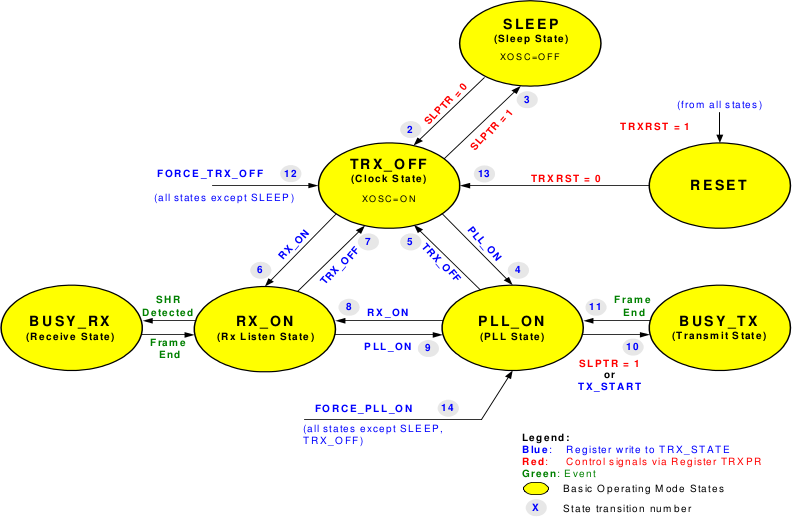
\includegraphics[width=\textwidth]
		{img/transceiver_operating_modes.png}
	\end{center}
	\caption{\small \itshape{Transceiver operating
	modes\protect\footnotemark}}
\end{figure}
\footnotetext{Image taken from ATmega128RFA1 datasheet. Copyright 2012 Atmel
Corporation.}

The two methods of interaction allow for more flexible application design.
The device can easily be integrated in both procedural and event-based systems.

The module uses double-buffering for frame data. There is an application frame
buffer and a transceiver frame buffer. Data is transferred between the two
buffers by the module's transmission and reception functions.

\section{Symbol counter}

The symbol counter module provides an interface for enabling and interacting
with the ATmega128RFA1 MAC symbol counter, which is used as the primary time
source in Sparrow-based applications. It allows the user to set two independent
timeouts as large as 4294967296 seconds and put the microcontroller to sleep
for up to 4294967296 milliseconds. As with the radio, the symbol counter module
provides two callbacks that can be called when one of the timeouts expires.

\lstset{
	language=C, numbers=none, caption=Time critical action snippet,
	label=lst:scounter_snippet
}
\begin{lstlisting}
#define TIMEOUT	30

void timeout_callback()
{
	do_time_critical_work();
	scounter_set_timeout(TIMEOUT, 0, OCR1);
}

int main()
{
	scounter_init(timeout_callback, NULL);
	scounter_set_timeout(TIMEOUT, 0, OCR1);

	while (1)
	{
		do_non_time_critical_work();
	}

	return 0;
}
\end{lstlisting}

\section{Debugging}

Though unessential, the debugging module is certainly one of the most useful.
It provides methods of configuring a debug interface and printing information
through it. Furthermore, debugging functionality can be enabled and disabled
through the build system, thus the programmer does not need to modify the code
in order to change to a release configuration. Simply deactivating the debug
option and regenerating the makefiles will cause the build process to generate
debug-free code.

% ********** End of Software platform **********
